\documentclass{article}
\usepackage{amsmath}
\usepackage{amsthm}
\usepackage{amsfonts}
\usepackage[a4paper,inner=30mm,outer=30mm,top=20mm,bottom=40mm]{geometry}
\usepackage{graphicx}

\title{An efficient numerical integration scheme for clonal expansion processes on graphs}
\author{Chay Paterson${}^\star$, Miaomiao Gao(?), Joshua Hellier(?), Ruibo Zhang(?), Georg Luebeck, David Wedge${}^\star$, Ivana Bo\v{z}i\'{c}}
% NB: order of authors subject to change but David and Ivana should be senior
% Affiliations: Manchester, DTSL, UW, The Hutch
% Limit: 10kw including figure captions

\begin{document}

\maketitle

\begin{abstract}
Compound birth-death processes are widely used to model the age-incidence curves
of many cancers \cite{luebeck2013impact}. There are efficient schemes for
directly computing the relevant % also cite Armitage and Doll
probability distributions in the context of linear multi-stage clonal expansion
(MSCE) models \cite{meza2008age}. These schemes have not been generalised to
models to arbitrary graphs, forcing the use of full stochastic simulations or
mean-field approximations, which can become inaccurate at late times or old ages
\cite{cpaterson2020,Paterson2021vs}.
Here, we present a numerical integration scheme for directly computing survival
probabilities of a first-order birth-death process on an arbitrary
directed graph, without the use of stochastic
simulations. As a concrete example, we use this new numerical method to analyse
historical data on copy number alterations in retinoblastoma. (TODO!)
\end{abstract}
% Key references: K Crump 2005, G Luebeck 2013, Connolly 2003

\section{Introduction}

% Basic problem: age and cancer risk. Can be modelled as incidence/hazard
% function or as a cumulative incidence/risk/probability in a reference
% population. The former is more useful for cohort-specific data.
The relationship between age and cancer incidence has provided crucial
biological insights since it was first noted by Armitage and Doll
\cite{armitage_doll,armitage1957two,knudson1971mutation}. It was 
recognised that the incidence could be modelled as the hazard function of a
compound random process, with multiple successive steps corresponding to
accumulating mutations in a population of pre-neoplastic cells
\cite{armitage_doll,moolgavkar1979two}. This class of mathematical models
established a paradigm for studies of cancer, age, and public health; resulting
in the discovery of tumour suppressor genes, and allowing detailed,
cohort-specific models of environmental risk factors
\cite{knudson1971mutation,conolly2003biologically,meza2008age}. 

The most sophisticated
models now incorporate selection and cell turnover in detail, and allow
inferences about the likely number of ``hits'' involved in the initiation of a
given type of cancer to be drawn from data on patient age \cite{moolgavkar1992multistage,luebeck2013impact}. These multi-stage clonal expansion (MSCE) models include four types of process:

% TODO copy over from old paper
\begin{itemize}
    \item Mutation (by asymmetric division): $j \rightarrow j + k$, at rate
    $\mu_j N_j$
    \item Birth (by symmetric division): $j \rightarrow j + j$, at rate
    $\alpha_j N_j$
    \item Death: $j \rightarrow \emptyset$, at rate $\beta_j N_j$
    \item Immigration: $\emptyset \rightarrow j$, at rate $\kappa_j$
\end{itemize}
labelling different cell types $j$ and $k$, and the numbers of these types $N_j$
and $N_k$, respectively. In most existing MSCE models, the different cell types $j$
and $k$ represent stages in a linear progression, and are indexed with
integers \cite{moolgavkar1992multistage,luebeck2013impact}. In more recent work,
the types $j$ are considered as nodes on a directed graph, to distinguish
between different mutational mechanisms, such as point mutations and copy number
alterations \cite{patersonbozic2020colorectal,Paterson2022}.

% \vec{N} for short?

There are thus four possible types of event for each subpopulation $N_j$: mutation,
birth, and death obey first-order kinetics, and immigration obeys zeroth-order
kinetics. The quantity of the most interest is
the probability $P(t,N_f > 0)$ that the final subpopulation $N_f$ is greater than
zero by a given age
$t$, interpreted as the likelihood that a population of neoplastic cells has emerged.
The probability $P(t,N_f > 0)$ is usually computed via $P(t,N_f > 0) = 1 - P(t,N_f = 0)$.
From this, one can define the hazard function $h(t)$,

\begin{equation}
    h(t) = \frac{d \ln P(t,N_f > 0)}{dt} = \frac{d \ln(1 - P(t,N_f = 0))}{dt}
\end{equation}
which models the age-related incidence \cite{luebeck2013impact}. We can
identify the probability to have \emph{no} cancerous cells $P(t,N_f = 0)$ with
the standard survival function $S(t)$.

TODO draw on Ivana's review?

% Summarise literature, Luebeck and Moolgavkar's work
As a class of stochastic process, probabilities (and thus hazard functions) for 
these models can be computed in a natural way by sampling many replicates of 
stochastic simulations using e.g. Gillespie's algorithm. However, a full
stochastic simulation is computationally expensive. Using sampling to estimate 
a probability $P$ with a standard error $\sigma$ of less than $\sigma < \epsilon$ 
requires on the order of
$P (1 - P) \epsilon^{-2}$ replicates, which grows rapidly as the error tolerance $\epsilon$
decreases.
A method to directly estimate $P(t,N_f = 0)$ or $h(t)$ numerically, given some
set of model parameters, is therefore highly desirable for the purposes of
statistical fitting. 
% Full stochastic simulation expensive

% Direct computation of the distribution or PGF desirable
% Reduction to quadrature possible
In fact, $n$-step MSCE models have well-studied methods
for reducing the computation of $P(t,N_f = 0)$ to numerical quadrature
\cite{moolgavkar1992multistage,crump2005numerical,meza2008age,luebeck2013impact}.
These methods represent $P(t,N_f = 0)$ (or $S_n(t)$,
conventionally) as a particular value of a generating function, conventionally 
denoted $\Psi$ or $\Phi$, and making use of Kolmogorov backward equations to derive
recursive formulae for the probabilities $S_n(t)$
\cite{crump2005numerical,moolgavkar1979two}. The probabilities $S_n(t)$ may then
be evaluated using an numerical integration scheme such as Gaussian quadrature
\cite{luebeck2013impact}. Kolmogorov forward equations have been less
well-investigated for this purpose compared to Kolmogorov backward equations.

% But these models can't distinguish between different mechanisms
% A robust generalisation to graphs/networks is desirable, but most existing
% schemes for networks have relied on mean field approximations or similar
% Also mention moment closure
% Citations: R. Grima and Winkelmann/Schutte

One common shortcoming of existing methods is that the mutational transitions are 
limited to linear graphs, or path graphs. More general models involving
birth-death-mutation processes on arbitrary directed graphs have previously only
been studied using stochastic simulations, or approximate solutions derived
from mean-field or moment closure approximations
\cite{patersonbozic2020colorectal,grima2010effective}.
Here, we define a numerical scheme based on Kolmogorov \emph{forward} equations
and the method of characteristics that is suitable for studying clonal expansion
models with constant coefficients on
arbitrary directed graphs \cite{crump2005numerical,quinn1989calculating}.

\section{Method}

% Summarise what we want to do

% Define graph in terms of vertex set V and edge set E
Different vertices in $V$ correspond to subpopulations with different
combinations of genetic alterations. Each subpopulation $N_j$, $j \in V$, is a
random variable. The initial value of $N_j$ at age $t=0$ will be denoted $Z_j$.
% Populations N_j are random variables with initial values Z_j, j in V

There is also a subset of nodes $F \in V$ which are ``final'' subpopulations. These
are interpreted as neoplastic or cancerous cells. Our overarching goal is to
compute the probabilities that chosen final nodes $f \in F$ are
unoccupied by time $t$: $P(t, N_f = 0)$.

%(Kinetics and an example graph)
% EXAMPLE GRAPHS:
\begin{figure}
    \caption{Left: an example of a two-step multi-stage clonal expansion
    model (MSCE). Right: a generalised MSCE on a directed acyclic graph,
    demonstrating how two different mechanisms of tumour suppressor loss can be
    incorporated in a graphical model. The two mechanisms in question are
    single-nucleotide variants on different alleles, and copy number loss on the
    locus. Adapted from \cite{Paterson2022}.}
\end{figure}

There are four processes through each cell population $N_j$ can change: birth
$\alpha_j$, death $\beta_j$, immigration $\kappa_j$, mutation $\mu_{jk}$. Each
coefficient is a non-negative real number. In terms of cell types $j \in V$, $k \in V$:

\begin{itemize}
    \item Mutation (by asymmetric division): $j \rightarrow j + k$, at rate
    $\mu_{jk} N_j$
    \item Birth (by symmetric division): $j \rightarrow j + j$, at rate
    $\alpha_j N_j$
    \item Death: $j \rightarrow \emptyset$, at rate $\beta_j N_j$
    \item Immigration: $\emptyset \rightarrow j$, at rate $\kappa_j$
\end{itemize}

In general, the rate coefficients $\{\alpha_j, \beta_j, \mu_{jk},
\kappa_j\}$ may vary with respect to age/time. However, in this work, the
special case where they are constant will be given special consideration, as
some dramatic optimisations are then possible.
% Ensure that the correct stoichiometry is used for mutation: asymmetric
% division

The edge set $E$ corresponds to pairs of nodes for which the mutation rate
$\mu_{jk} > 0$, and are interpreted as different mutational mechanisms. These may be
mutations on different loci, or different biological processes such as
deletions, loss of heterozygosity, copy number alterations and so on. 
e.g. the graph may be a tree, with different vertices representing different
ancestral genotypes.

The set of nodes $V$ and edge set $E$ together define a graph $G=(V,E)$
\cite{intrographs}.

These dynamics imply the following general form for the Kolmogorov forward
equations:
% Kolmogorov forward equations, in general
\begin{align}
    \frac{d P(t, N_0, N_1, \dots)}{dt} &=
    \sum_{j \in V} \left(
    \alpha_j (N_j - 1) P(t, N_0, \dots, N_j - 1, \dots)
    + \beta_j (N_j + 1) P(t, N_0, \dots, N_j + 1, \dots)
    \vphantom{\sum_a^b}
    \right.
    \nonumber \\
    &\quad \left. + \sum_{k \in V} \mu_{kj} N_k P(t, N_0, \dots, N_k, \dots,  N_j - 1, \dots)
    + \kappa_j P(t, N_0, \dots, N_j - 1, \dots)
    \right.
    \nonumber \\
    &\quad \left. 
    - \left(\alpha_j N_j + \beta_j N_j + \sum_{k \in V} \mu_{jk} N_j + \kappa_j\right)
    P(t, N_0, \dots, N_j, \dots)
    \vphantom{\sum_a^b}
    \right)
    \label{eq:kolmogorov}
\end{align}

% Group these into a sum over vertices, annotate the immigration, birth, death,
% and mutation processes
% Generating function \Psi: transforms into a PDE, wave equation

We define the generating function $\Psi$ to be the expected value of $\prod_{j \in V}
q_j^{N_j}$ given some tuple of conjugate coordinates $\vec{q} = \{q_0, q_1, \dots\} \in
\mathbb{C}^n$ \cite{gfology}.

\begin{equation}
    \Psi(t,q_0,q_1,\dots,q_j,\dots) 
    = \mathbb{E}\left[\prod_{j \in V} q_j^{N_j}\right]
    = \sum_{N_0 = 0,\dots,N_j=0,\dots}^{N_0 = \infty,\dots, N_j = \infty, \dots} \prod_{j \in V} q_j^{N_j} 
        P(t, N_0, \cdots, N_j, \cdots)
\end{equation}
where the sum runs over all possible values of the populations $\vec{N} = \{N_0,
N_1, \cdots, N_j, \cdots\}$.
One can note that this is essentially the Fourier transform of the probability
distribution $P(t,N_0,\dots)$ with respect to the variables $N_j$. The variables
$q_j$ are conjugate to the populations $N_j$, forming Fourier duals in the same
sense as frequency and time.

The probability $P(t,N_f = 0)$ that some population $N_f = 0$ at age $t$ can
then be expressed in terms of $\Psi$:

\begin{equation}
    \Psi(t,1,1,\dots,q_j = 1,\dots, q_f = 0)
    = \sum_{N_0 = 0,\dots,N_j=0,\dots}^{N_0 = \infty,\dots, N_j = \infty, \dots}
        P(t, N_0, \cdots, N_j, \cdots, N_f = 0)
    = P(t,N_f = 0)
    \label{eq:corner}
\end{equation}
i.e. set $q_j = 1$ for all $j \neq f$, and $q_f = 0$.

When recast in terms of the generating function $\Psi$, equation
\eqref{eq:kolmogorov} becomes a partial differential equation

\begin{align}
    \frac{\partial \Psi}{\partial t} &= 
    \sum_{j \in V} \left(
    \left(
    \alpha_j (q_j - 1)
    + \beta_j (q_j^{-1} - 1)
    + \sum_{k \in V} \mu_{jk} (q_k - 1) 
    \right) q_j \frac{\partial  \Psi}{\partial q_j}
    +\kappa_j (q_j - 1)  \Psi \right)
    \nonumber \\
    &= \sum_{j \in V} X_j(\vec{q}) \frac{\partial \Psi}{\partial q_j}
    + Y(\vec{q}) \Psi 
    \label{eq:wave}
\end{align}
where

\begin{equation}
    X_j(\vec{q}) :=
    \alpha_j (q_j - 1) q_j
    + \beta_j (q_j^{-1} - 1) q_j
    + \sum_{k \in V} \mu_{jk} (q_k - 1) q_j
\end{equation}
\begin{equation}
    Y(\vec{q}) = \sum_{j \in V}\kappa_j (q_j - 1)
\end{equation}
% Define the generating function as the expectation of \prod_{j \in V} q_j^{N_j}
% Note that this generalises other definitions in the literature

% Note that the question we want to answer for S_n(t) has some specific q_j
% coordinates
The quantity we want to solve for, $P(t,N_f = 0)$, has an associated set of
$\vec{q}$ coordinates:

\begin{equation}
    \vec{q} = (q_0,q_1,q_2,\dots,q_f) = (1,1,1,\dots,0)
\end{equation}
or

\begin{equation}
    q_j = 1 - \delta_{j,f}
\end{equation}
where $\delta_{ij}$ is the Kronecker delta symbol.

\subsection{Formal solution by the method of characteristics}

\subsection*{Theorem:}

%(t, \vec{q})

A general solution to \eqref{eq:wave} is given by
\begin{equation}
    \Psi(t,q_0,q_1,\dots) = \left(\prod_{j \in V}
    \gamma_j(\sigma=t)^{Z_j}\right)
    e^{\int_{\sigma=0}^t Y(\vec{\gamma}(\sigma)) d\sigma}
    \label{eq:formalsln}
\end{equation}
where the characteristics ${\gamma}_j$ are solutions of the initial value problem

\begin{align}
    \frac{d {\gamma}_j}{d \sigma} &= {X}_j(\vec{\gamma}),
    \nonumber \\
    {\gamma}_j(\sigma = 0) &= {q}_j
    \label{eq:ivp}
\end{align}
where the vector field $\vec{X}$ and scalar field $Y$ are defined to be

\begin{equation*}
    X_j(\vec{\gamma}) :=
    \alpha_j (\gamma_j - 1) \gamma_j
    + \beta_j (\gamma_j^{-1} - 1) \gamma_j
    + \sum_{k \in V} \mu_{jk} (\gamma_k - 1) \gamma_j
\end{equation*}
and
\begin{equation*}
    Y(\vec{q}) = \sum_{j \in V}\kappa_j (q_j - 1)
\end{equation*}
and $\vec{\gamma}$ is shorthand for $(\gamma_0, \gamma_1, \cdots, \gamma_j,
\cdots)$.

Values of $\Psi$ can thus be computed for any given set of initial conditions
$\vec{q}$. As an immediate corollary, this allows $P(N_f = 0)$ to be calculated:
the relevant initial conditions are given by \eqref{eq:corner}, with $q_j = 1$
for all $j\neq f$, and $q_f = 0$.

\subsection*{Proof}

The wave equation \eqref{eq:wave} can be placed into a conservation form along a vector field
$\vec{X} = (X_0,X_1,\cdots,X_j,\cdots)$:

\begin{equation}
    \frac{\partial \Psi}{\partial t} = \vec{X}(\vec{q}) \cdot \nabla \Psi + Y(\vec{q}) \Psi
    \label{eq:wave2}
\end{equation}
This can be solved using the method of characteristics. Briefly, we seek a
parametrised family of curves $\tau(\sigma)$, $\vec{\gamma}(\sigma)$ for which

\begin{equation}
    \frac{d \Psi}{d \sigma} = \frac{d \tau}{d \sigma} \frac{\partial \Psi}{\partial t} 
    + \sum_{j \in V} \frac{d \gamma_j}{d \sigma} \frac{\partial \Psi}{\partial q_j}
\end{equation}
and $\tau(0) = t,\vec{\gamma}(0) = \vec{q}$. An appropriate family of curves is
\begin{align}
    \frac{d \tau}{d \sigma} &= -1
    \nonumber \\
    \frac{d \vec{\gamma}}{d \sigma} &= \vec{X}
    \nonumber
\end{align}
Clearly $\tau(\sigma) = t - \sigma$. The characteristics
$\vec{\gamma}=(\gamma_0,\gamma_1,\cdots)$ will have a more complicated form.

Along these curves, equation
\eqref{eq:wave2} takes the form

\begin{equation}
    \frac{d \Psi}{d \sigma} = -Y(\vec{\gamma}) \Psi
    \label{eq:this}
\end{equation}
where
\begin{equation}
    Y(\vec{\gamma}) = \sum_{j \in V}\kappa_j (\gamma_j - 1)
\end{equation}
Integrating \eqref{eq:this} and rearranging for $\Psi(\tau(0) = t, \vec{\gamma}(0) =
\vec{q})$ yields

\begin{equation}
    \Psi(\tau(0) = t, \vec{\gamma}(0) = \vec{q})
    = \Psi(\tau(\sigma = t) = 0, \vec{\gamma}(\sigma = t))
    \exp\left(\int_{\sigma=0}^t Y(\vec{\gamma}) d\sigma\right)
\end{equation}
Given that the initial conditions are known,

\begin{equation}
    \Psi(0, \vec{\gamma}(\sigma=t)) = \prod_{j \in V} \gamma_j(\sigma=t)^{Z_j}
\end{equation}
Substituting this results in the formal solution \eqref{eq:formalsln}.

% So we can instead ask about a final value problem involving the
% characteristics \vec{\gamma}
% This gets us a formal solution for \Psi

\subsection{Geometrical interpretation}

The flow $\vec{X}$ has an elegant geometrical interpretation: although we
assumed that each $q_j$ coordinate was in general, a complex variable of
arbitrary norm, the $q_j$ coordinates naturally describe points in a real unit
cube, henceforth $Q$. The vector field $\vec{X}$ describes a flow on this cube, and the
scalar function $Y$ describes an absorption term. Equation \eqref{eq:wave} can
therefore be seen as a transport equation: the quantity $\Psi$ is transported
through the cube by $\vec{X}$.

The initial conditions implied by \eqref{eq:corner} lie at one of the corners of
this cube.

(Conceptual diagram of this flow)

When considered as a dynamical system on the cube $Q$, a number of properties
of MSCE models become apparent.

The form of $\vec{X}$ ensures that $Q$ is a ``trapping region'' of the
vector field. At every point on the boundary $\partial Q$, $\vec{X}$ points weakly
into $Q$. As a result, for all initial conditions of $\vec{q} \in Q$ on its
boundary $\partial Q$ will end up somewhere inside $Q$ in a finite time, and will never leave.

To see this, examine $\vec{X}$ on the boundary $\partial Q$, which are those
points with all $q_j \in [0, 1]$. At $q_j = 0$,

\begin{equation*}
    X_j = +\beta_j \geq 0
\end{equation*}
which points into the interior of $Q$, and at $q_j = 1$,

\begin{equation*}
    X_j = \sum_{k \in V} \mu_{jk} (q_k - 1) \leq 0
\end{equation*}
because $\mu_{jk} \geq 0$.

Finally, at the point $(q_0, q_1, \dots, q_k) = (1,1,\dots,1)$, where $q_j=1$
for all $j$, it is easily seen that $\vec{X} = \vec{0}$, and this point is thus
an equilibrium.

% Cute conceptual diagram
\begin{figure}
    % Left view | Right view
    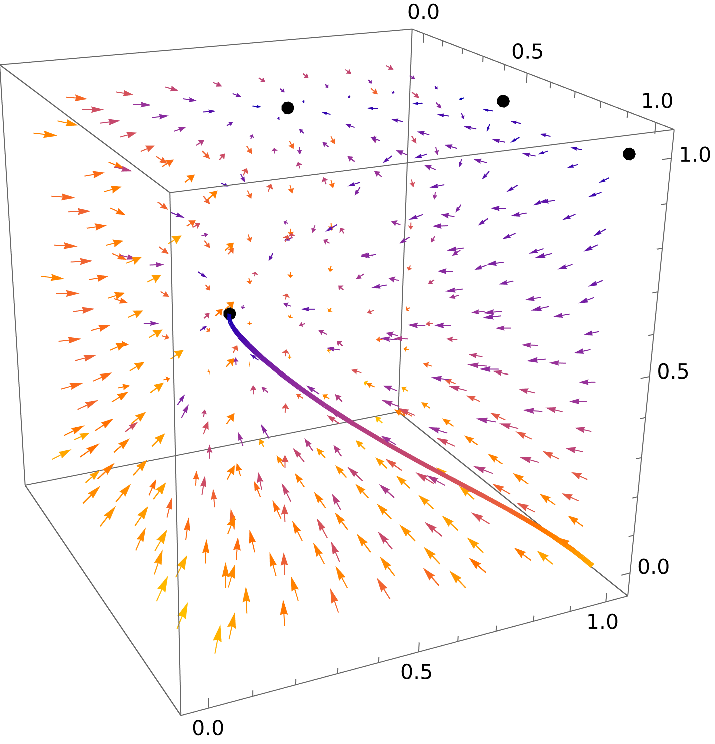
\includegraphics[width=0.5\textwidth]{figures/flowcube1}
    % Below:
    \caption{\label{fig:cube}Above: an example of the flow $\vec{X}$ imposed on the
    conjugate coordinates $\vec{q}$ by equation \eqref{eq:wave}. This represents
    a three-stage model on a linear graph $0 \rightarrow 1 \rightarrow 2$ (Below), with rates $\alpha_j = 2.0, \beta_j = 1.0, \mu_{01} = \mu_{02} = 1.0$. As
    there are three nodes, the conjugate coordinates $\vec{q}=(q_0,q_1,q_2)$
    describe a cube. Three equilibria are visible: one at the corner $(1,1,1)$,
    two additional equilibria on the cube boundary with $q_2 = 1$, and
    an interior equilibrium at $\vec{q}^\star = (0.337143, 0.359612, 0.5)$, representing the
    probability of survival of a cell placed on sites $0$, $1$ and $2$. The characteristic
    curve $\vec{\gamma}$ with initial conditions $(1,1,0)$ has also been
    plotted: this would be used to calculate the probability $P(t,N_2 = 0)$ with
    the algorithm detailed in section \ref{sec:flying}.}
\end{figure}

% Form of generalised solution immediately implies Meza and Luebeck's
% observations about different regimes:
The form of the vector field $\vec{X}$ also implies that several early results
of Armitage and Doll hold much more generally, as well as Meza and Luebeck's observations about different qualitative regimes of the hazard function\cite{armitage1957two,meza2008age}. Recall that the relevant initial condition \eqref{eq:corner} to compute $P(N_f = 0)$ was $q_0 = 1, q_1 = 1, \cdots, q_f = 0$.  At this corner, $\vec{X}$ degenerates to

\begin{align}
    X_j &= - \mu_{jf}, \quad j \neq f
    \nonumber \\
    X_f &= + \beta_f
\end{align}
Although we haven't made an explicit assumption about the structure of the graph
$G$, most entries of $\mu_{jf}$ will be zero: only terms corresponding to edges
connecting the final node $f$ to other vertices $j$ on the graph $G$ will have
nonzero $\mu_{jf}$. Consider a node $j$ just next to $f$, so that the edge
corresponding to $\mu_{jf}$ points from $j$ into $f$.

% Diagram:
% j --> f
% TODO diagrams in dot?
The initial conditions at this $j$ are $\gamma_j = q_j = 1$. Furthermore, $d
\gamma_j / d\sigma = -\mu_{jf}$. So, to leading order, $\gamma_j = 1 -
\mathcal{O}(t)$.

% Gist: P(N_f = 0) to first order is 1 - O(t^n)

...

It therefore follows that to leading order, 
\begin{equation}
    P(t, N_f = 0) = 1 - \mathcal{O}(t^n)
\end{equation}
at sufficiently short times $t$. This expresses the classic dependence of
Armitage and Doll \cite{armitage_doll}.

The asymptotic behaviour at very long times also immediately demonstrates the
long-term exponential regime noted by Luebeck and Meza \cite{meza2008age}.
It can be shown that as well as the equilibrium at the point $\vec{q} =
(1,1,1,\dots,1)$, there is a second equilibrium point $\vec{q}^\star$ inside $Q$ (see appendix 2
for a proof). Furthermore, $\vec{q}^\star$ is isolated, and $Q$ is a trapping region:
all paths $\vec{\gamma}$ should head towards $\vec{q}^\star$.

Around $\vec{q}^\star$, $\vec{X}$ can be linearised, and the characteristics
$\vec{\gamma}$ will obey

\begin{equation}
    \vec{\gamma} \approx \vec{q}^\star + \sum_i \vec{c}_i e^{\lambda_i t}
\end{equation}
where the sum is taken over eigenvalues $\lambda_i$, and $\vec{c}_i$ depends on
initial conditions. If $G$ is acyclic, the eigenvalues $\lambda_i$ must be real
and negative (see appendix 2). The various $\gamma_j$ will then relax towards
the equilibrium exponentially, the same behaviour described by Luebeck and
Moolgavkar in a different framework \cite{meza2008age}.

It follows that the probability $P(t,N_f = 0) = \Psi(t, 1,1,\dots,q_f = 0)$ also
has an asymptote. Suppose that all $Z_i$ cells initially start on some node $i \in
V$, and there is no immigration. Then:

\begin{equation}
    \lim_{t\rightarrow \infty} P(t, N_f = 0) = 
    \lim_{t\rightarrow \infty} \Psi(t,1,1,\dots,q_f=0) =
    \left(q^\star_i\right)^{Z_i}
\end{equation}
This allows a more concrete interpretation to the conjugate variables $q_j$,
which are more abstract than the populations $N_j$: the
quantity $q^\star_i$ corresponds to the probability that a single cell on the
starting node $i$ will never produce a cancerous cell of type $f$, because its lineage goes
extinct. The fact that birth, death, and mutation are all first-order processes
implies that there are $Z_0$ independent trials.

In general, with multiple independent initial populations $Z_j$, we have 
\begin{equation}
    \lim_{t\rightarrow \infty} P(t, N_f = 0) = 
    \lim_{t\rightarrow \infty} \Psi(t,1,1,\dots,q_f=0) =
    \prod_{j \in V} \left(q^\star_j\right)^{Z_j}
\end{equation}
Each equilibrium conjugate coordinate $q^\star_j$ therefore corresponds to the
probability that the lineage of a single cell on node $j$ goes extinct. The
conjugate coordinates can therefore be thought of as ``survival probabilities''.
It is easily verified that each $q^\star_j \rightarrow 0$ as 
$\beta_j \rightarrow 0$, as would be expected.

\subsection{Numerical integration schemes}



\subsection*{Non-constant coefficients: Quinn's method}
% Need to treat t as a constant
% Quinn's method: two-pass procedure
% Cache new characteristics for each value of t
% Compute theta = \int Y d\sigma afterwards using cached \gamma_j
When the coefficients $\{\alpha_k(t), \beta_k(t), \kappa_k(t), \mu_{jk}(t)\}$
have an explicit time dependence, the following scheme by Quinn can be used\cite{quinn1989calculating}. Explicit time dependence is relevant to e.g. tobacco smoking
and possibly inflammatory conditions linked to pre-cancer (Barrett's oesophagus and maybe
EBV and lymphoma?). In the following, the coefficients are assumed to have a
specified functional form, and e.g. $\alpha_j(t)$ represents a function call.

For each value of $t$, new characteristic curves $\gamma_j(\sigma)$ (with initial
conditions $q_j$) and weights
$w = \int Y(\vec{\gamma}(\sigma)) d\sigma$ are computed in a ``two pass'' procedure, using Euler
integration to update the $\gamma_j$, and the rectangle rule to update the
weights. These
characteristic curves can then be substituted into \eqref{eq:formalsln}, and
corresponding values for $P(N_j = 0)$ computed.

(...TODO rewrite in proper pseudocode environment...)

\begin{enumerate}
    \item Choose and fix a time step $\Delta t$.
    \item For each time of interest $t$...
    % indent {
    \item Initialise $\sigma = 0$, $w = 0$ and $\gamma_j = q_j$ for all $j$.
    \item While $\sigma < t$:
    % indent {
    \item Update $\gamma_j \leftarrow \gamma_j + X_j \Delta t$ for all $j$.
    (Euler integration)
    \item Update $w \leftarrow w + Y(\vec{\gamma}(t)) \Delta t$.
    \item Update $\sigma \leftarrow \sigma + \Delta t$.
    \item Store the values $(\vec{\gamma}, \sigma)$.
    % indent }
    \item Using the cached values of $(\vec{\gamma}, \sigma)$ compute $\int_{\sigma=0}^t
    Y(\vec{\gamma}(\sigma)) d\sigma$ and hence $\Psi(t, \vec{q})$.
    % indent }
\end{enumerate}


For any explicit time-stepping procedure with step size $\Delta t$, the number
of operations to compute one of these characteristic curves will be $N = \lceil
t_{max} / \Delta t \rceil$. To compute values of $P(N_j = 0)$ at all $N$ times
in between $t=0$ and $t=t_{max}$ will therefore require $\mathcal{O}(N^2)$
operations. This is explicitly described in Crump's review and Quinn's original
paper \cite{crump2005numerical,quinn1989calculating}.

\subsection{Constant coefficients: a one-pass method}
\label{sec:flying}
% Flying conjugates
% ask what happens as we advance t -> t + \Delta t
% to advance \Psi by \Delta t, we just have to update the characteristics and
% \theta = \int Y d\sigma

Inspecting the formal solution \eqref{eq:formalsln} immediately
suggests other numerical schemes along the lines of Quinn's. We will describe a simple
implementation based on \emph{improved} Euler integration and the rectangle rule: more
sophisticated schemes are obviously possible.
However, when the coefficients $\{\alpha_k, \beta_k, \kappa_k, \mu_{jk}\}$ are
independent of time, a more radical optimisation of Quinn's method is possible.

Consider what happens to \eqref{eq:formalsln} when $t$ is replaced by $t +
\Delta t$, where $\Delta t$ is a finite time step. Equation \eqref{eq:formalsln}
must be valid at all times, so it should be true that

\begin{equation}
    \Psi(t + \Delta t,q_0,q_1,\dots) = \left(\prod_{j \in V}
    \gamma_j(\sigma=t + \Delta t)^{Z_j}\right)
    e^{\sum_{j \in V} \int_{\sigma=0}^{t + \Delta t} \kappa_j (\gamma_j(\sigma)-1) d\sigma}
\end{equation}
Each characteristic solves \eqref{eq:ivp}, so

\begin{equation}
    \gamma_j(t+\Delta t) = \gamma_j(t) + \int_{t'=t}^{t+\Delta t} X_j dt'
\end{equation}
which can be computed with an appropriate numerical integration procedure, for
example improved Euler integration:

\begin{align}
    \tilde{\gamma_j} &= \gamma_j(t) + X_j(\vec{\gamma}) \Delta t \nonumber \\
    \gamma_j(t+\Delta t) &\approx \gamma_j(t) + \frac{\Delta t}{2}
    (X_j(\vec{\gamma}) + X_j(\tilde{\vec{\gamma}}))
\end{align}
(or an improved relative such as a higher-order Runge-Kutta, etc.).

The remaining term can also be approximated numerically. For brevity, call

\begin{equation}
    w(t) := {\sum_{j \in V} \int_{\sigma=0}^{t} \kappa_j (\gamma_j(\sigma)-1) d\sigma}
\end{equation}
and notice that
\begin{align}
    w(t + \Delta t)
    &= w(t) +
    \sum_{j \in V} \int_{\sigma=t}^{t + \Delta t} \kappa_j (\gamma_j(\sigma)-1) d\sigma
    \nonumber \\
    &\approx  w(t) + \sum_{j \in V} \kappa_j (\gamma_j(t)-1) \Delta t
\end{align}
effectively approximating $w(t+\Delta t)$ with the rectangle rule.

This shows that the generating function $\Psi(t, \vec{q})$ can be computed
numerically, by applying a time-stepping procedure to the characteristics
$\vec{\gamma}$. A concrete implementation in pseudocode might be:

\begin{enumerate}
    \item Choose and fix a time step $\Delta t$ and maximum time $t_{max}$.
    \item Initialise $t = 0$, $w = 0$ and $\gamma_j = q_j$ for all $j$.
    \item Update $\gamma_j$ for all $j$ with an improved Euler step.
    \item Update $w \leftarrow w + \sum_{j \in V} \kappa_j (\gamma_j(t)-1)
    \Delta t$.
    \item Update $t \leftarrow t + \Delta t$.
    \item Compute $\Psi(t, \vec{q}) = \left(\prod_{j \in V}
    \gamma_j(t)^{Z_j}\right) e^w$.
    \item If $t$ is less than $t_{max}$, go to 3. Otherwise, exit.
\end{enumerate}

The only dynamical quantities that need to be stored and updated are $t$, the
weight $w$, and the
characteristics $\gamma_j$. A new value of $\Psi(t, \vec{q})$ may be computed
and returned at every time step. Only one set of characteristics need to be computed
between $\sigma = 0$ and $\sigma = t$ to get a complete set of values for
$\Psi$. This scheme will terminate after $N = \lceil t_{max} / \Delta t \rceil$
iterations. This is much faster than Quinn's method -- requiring
$\mathcal{O}(N)$ operations instead of $\mathcal{O}(N^2)$.

More sophisticated schemes are easy to imagine. For example, Euler integration
of the characteristics $\gamma_j$ could be replaced by improved Euler
integration or Runge-Kutta methods. The rectangle method for computing $w(t)$
could be replaced by the trapezoid rule, knowing $\gamma_j(t)$ and $\gamma_j(t +
\Delta t)$. And so on.

\section{Application to statistical inference: maximum likelihood parameter estimation}

Problem: given a set of observations of the times $t_i$ at which a cancer
appeared of type $f_i$, what are the best possible estimates of the underlying
parameters $\theta = \{\alpha_j, \beta_j, \kappa_j, \mu_{jk}\}$ ?

The exact time at which the first cancerous cell emerged in a patient is
unobservable. The data we do have access to is censored to the left:
we know the patient's age when the cancer was detected, $t_i$, which gives us an
upper bound on the time the cancer appeared. All that this tells us is that at
the time of detection, the number of cancer $N_{f_i}$ cells was greater than
zero. The corresponding probability is therefore $P(t_i, N_{f_i})$.

The corresponding likelihood of observing the whole dataset $\{t_i,f_i\}$, given
the parameters $\theta$, is thus

% Likelihood of a dataset = prod_i P(t_i, N_f_i = 0)

\begin{equation}
    \mathcal{L}(\theta | \{t_i, f_i\}) = \prod_i 
    \left. (1 - P(t, N_{f_i} = 0)) \right|_{t=t_i}
\end{equation}
Maximising this likelihood with respect to the parameters
$\theta = \{\alpha_j, \beta_j, \kappa_j, \mu_{jk}\}$ will produce best estimates
for those parameters.
This can be done by a number of methods, now that we have an efficient scheme
for computing $P$: e.g. gradient descent/ascent, which can be simplified by
using analytical expressions for the scores $\nabla_\theta \gamma_j$ (basically
backpropagation). Or simulated annealing
% Basically, use \nabla_\theta X_j and \gamma_j to evolve the auxiliary
% variables \nabla_theta \gamma_j along the characteristics.
% The characteristic curves \gamma_j and auxiliary terms form a "fiber bundle"
% which is nice geometrical flavour.

\begin{equation}
    \frac{d \nabla_\theta \gamma_j}{d \sigma} = \nabla_\theta X_j
\end{equation}

\section{Results}

Compare to Gillespie for 2-hit model.

  Conclusions: very fast

Compare to Gillespie for the CRC model

  Must agree

  Must be faster

% Maybe: examine correlations on 3 different 2-hit trees
%   parallel a->b->c
%            d->e->f
%   distant MRCA: a->b->c
%                 a->e->f
%   recent MRCA:  a->b->c
%                 a->b->f
% Examine correlations between c and f. This is impossible in the mean-field
% approximation, which assumes that all populations are uncorrelated.
%
% Hypothesis: if b has a fitness advantage, we should see strong correlations in
% the last case and low or zero correlations in the previous two cases.

\subsection{Comparison of methods}

TODO Ruibo's data?

\subsection{Inverse problem: performance of maximum likelihood optimisation}

TODO retinoblastoma data?

Maybe leave this for future work?

\begin{figure}
\begin{tabular}{|c|c|c|c|c|}
\hline
Algorithm & Parameter values & Compiler flags & Runtime & Standard deviation \\
\hline
\end{tabular}
\caption{Table showing performance of the Gillespie algorithm and our novel
one-pass adaptation of Quinn's algorithm detailed in section \ref{sec:flying}. A
range of coefficient values are explored. All computations were carried out on
an AMD Ryzen 5 3600XT CPU, and compiled with GCC 12.2.0.}
\end{figure}

\section{Discussion}

% Should enable more efficient numerical estimates and fitting procedures for
% network models of cancer.
% This in turn should allow more detailed molecular data, including copy number
% alterations and a variety of different genomic rearrangements, to be used in
% combination with epidemiology, connecting more diverse mechanisms.
%   Better estimates of parameters of biological mechanisms
%   Personalised medicine

The fast algorithm presented here should enable more efficient numerical
estimates regarding biological mechanisms relevant to carcinogenesis, and faster
inference and fitting procedures for network models of cancer. This in turn
should allow risk models based on detailed molecular data to be used in
combination with epidemiological data, such as locus-specific copy number
alterations and a variety of genomic rearrangements. These risk models should
capture more individualised risk factors, showing how predispositions interact
with patient age, which may have applications in personalised medicine.

Continued work is necessary to find a numerical integration algorithm for
evolution of graphs that is suitable for time-varying coefficients $\{\alpha_j,
\beta_j, \mu_{jk}, \kappa_j\}$, which are necessary for studying carcinogenesis
associated with inflammatory conditions and smoking. Quinn's algorithm of 1988
is one candidate, but there may be optimisations that have not yet been
explored, especially with regards to convergence speed and the amount of
necessary caching.

\section{Acknowledgements}

We would like to thank Clare Gratrex for productive discussions regarding the
method and related literature.

% Author contributions:
% G Luebeck referencing and background literature
% J Hellier numerics

\bibliographystyle{unsrt}
\bibliography{references}

\section{Appendix 1}

Other stoichiometries for mutation/migration reactions can also be considered.
In general, a first-order reaction of the form

\begin{equation}
    j \rightarrow m j + n k
\end{equation}
will result in a term

\begin{equation}
    (q_j^{m-1} q_k^n - 1) q_j \frac{\partial \Psi}{\partial q_j}
\end{equation}
in equation \eqref{eq:wave}.

\section{Appendix 2}

The vector field $\vec{X}$ has equilibria at points where all the components
$X_j = 0$ simultaneously. Consider any one of the $X_j$:
\begin{equation}
    X_j = \alpha_j (q_j^2 - q_j) + \beta_j (1 - q_j) 
          + \sum_{k \in V} \mu_{jk} (q_k - 1) q_j = 0
\end{equation}
In general, this will define a curve parametrised by the other $q_k$, the
$j^{th}$ nullcline.
This can be thought of as a quadratic equation in $q_j$, and as such will have
at most two real roots in $q_j$. We know that one of these roots will be at $q_j
= 1$, when all the $q_k = 1$ also. For $q_k$ on the interior of $Q$, there
should be another root, as we previously showed that $X_j$ has opposite signs at
$q_j = 0$ and $q_k = 1$. This can also be shown by direct computation: there
will be a second root in $q_j$ if the discriminant of the quadratic equation $\Delta > 0$.

Treating the other $q_k$, $k \neq j$ as algebraically independent parameters,
the discriminant $\Delta$ is

\begin{align}
    \Delta &= (-\alpha_j -\beta_j + \sum_k \mu_{jk} (q_k - 1))^2 - 4\alpha_j \beta_j
    \nonumber \\
    &= (\alpha_j - \beta_j)^2 - 2 (\alpha_j + \beta_j) \sum_k \mu_{jk} (q_k - 1)
    +(\sum_k \mu_{jk} (q_k - 1))^2
\end{align}
For any $0 < q_k < 1$, $(q_k - 1) < 0$.

Define $m = \mathrm{min}_E(\mu_{jk}) > 0$, with $E$ the set of edges defined by
$\mu_{jk}$, and $D = \|V\|$, the number of vertices on $G$. It follows that

\begin{equation}
    \sum_k \mu_{jk} (q_k - 1) \leq - m D < 0
\end{equation}
and it follows that

\begin{equation}
    \Delta \geq (\alpha_j - \beta_j)^2 + 2 (\alpha_j + \beta_j) m D + m^2 D^2 > 0
\end{equation}
As $\Delta > 0$, $X_j$ has exactly two roots in $q_j$. This argument holds for every
$j \in V$ independently, and as such there must be a unique second equilibrium on the
interior of $Q$.

% TODO: boundary equilibrium is not unique b.c. the quadratic is degenerate

Finally, at any point $\vec{q} \in Q$, the Jacobian $J$ of $\vec{X}$ will be

\begin{equation}
    J_{jl} = \left(\alpha_j (2 q_j - 1) - \beta_j + \sum_k \mu_{jk} (q_k - 1)
    \right) \delta_{jl} + \mu_{jl} q_j
\end{equation}
If $G$ is acyclic, then $\mu_{jk}$ will be lower triangular, and the eigenvalues
of $J_{jl}$ will be real.

The interior equilibrium point is isolated: positive eigenvalues would be
inconsistent with this equilibrium being unique, and with $Q$ being a trapping
region for $\vec{X}$. 

\end{document}
